\chapter{Analyse}
\graphicspath{{04-Analyse/}}
\minitoc
\section{Analyse de la relaxation}Le processus de relaxation utilisé dans l'algorithme CxSOM est une méthode originale pour construire des connexions bidirectionnelles entre cartes. Deux cartes connectées de cette façon jouent alors un rôle symétrique, contrairement à une connexion unidirectionnelle ou hiérarchique dans laquelle une carte joue le rôle d'entrée et une autre de sortie. Dans cette section, nous évaluons expérimentalement la méthode de relaxation en tant que moyen de trouver une best matching unit (BMU). On cherchera notamment à répondre aux questions suivantes :  
\begin{itemize}
\item Est-ce que la méthode de relaxation converge ?
\item Est-ce que que cette méthode permet de définir un unique BMU ?
\item Quels sont les paramètres à prendre en compte dans l'algorithme de relaxation ?
\end{itemize}

\subsection{Formalisation de la relaxation}

La relaxation est une recherche de point fixe de l'activité globale de chaque carte de l'architecture. Notons $(\mathbf{\bmu})_\tau = (\bmu\m{0}_\tau,\cdots,\bmu\m{N}_\tau)$ la suite définie par l'évolution des BMUs des $N$ cartes d'une architecture lors de la relaxation.
La suite $(\mathbf{\bmu})_\tau$ est une suite définie par récurrence par $\mathbf{\bmu}_{\tau+1} = \mathbf{f}(\mathbf{\bmu}_\tau)$
avec $\mathbf{f} = (f\m{0},\cdots,f\m{N}) : [0,1]^N \rightarrow [0,1]^N$ une application non linéaire transformant l'espace des positions des BMUs; $\mathbf{f}$ ne dépend pas de $\tau$.


Détaillons l'évolution de cette suite. Pour clarifier les notations, définissons pour chaque carte~$i$:
\begin{equation}
\begin{gathered}
p\star\m{i}_{\tau} = \argmax_{p\m{i}}(a_g\m{i}(p\m{i},\bmu\m{i_0}_\tau, \cdots \bmu\m{i_K}_\tau))\\
 i_0, \cdots i_K \: \text{indices des cartes nourrissant la carte $i$}.
\end{gathered}
\label{eq:pstar}
\end{equation}
$a_g\m{i}$ est une fonction des poids de la carte $\w\ext\m{i}, \w\cont\m{i}$ et de son entrée externe $\inpx\m{i}$. Lors du processus de relaxation, les poids et l'entrée restent fixes. Le calcul de $a_g$ ne dépend pas de $\tau$.
Pour toute carte $i$, $p\star\m{i}_{\tau}$ est donc seulement une fonction de $(\bmu\m{i_0}_\tau, \cdots \bmu\m{i_K}_\tau)$.
L'équation d'évolution s'écrit alors: 
\begin{equation}
\bmu\m{i}_{\tau+1} = 
\begin{cases}
\bmu\m{i}_{\tau} + sgn(p\star\m{i}_{\tau} - \bmu\m{i}_{\tau}) \times \delta \; & \text{si $p\star\m{i}_{\tau} - \bmu\m{i}_{\tau} > \delta$ } \\
p\star\m{i}_{\tau} \; \text{sinon}	
\end{cases}
\label{eq:evolution}
\end{equation}

En posant $f\m{i}$ la partie droite de l'équation \ref{eq:evolution}, on peut donc écrire: 
\begin{equation}
\bmu\m{i}_{\tau +1} = f\m{i}(\bmu\m{0}_\tau,\cdots,\bmu\m{N}_\tau)
\label{eq:fonction}
\end{equation}
Soit, pour l'ensemble des composantes : 
\begin{equation}
\mathbf{\bmu}_{\tau+1} = \mathbf{f}(\mathbf{\bmu}_\tau)
\end{equation}

La relaxation se traduit ainsi par une recherche de point fixe de la suite $(\mathbf{\bmu})_{\tau}$, soit une position $\mathbf{\bmu}$ telle que:
\begin{equation}
\mathbf{\bmu} = \mathbf{f}(\mathbf{\bmu})
\label{eq:suite}
\end{equation}

Si $f$ admet un point fixe, alors ce point fixe est aussi un point fixe pour la suite $(\mathbf{\bmu})_\tau$. Cependant, rien ne garantit que ce point fixe existe, et qu'il sera atteint par la suite. Expérimentalement, il semble que si $\mathbf{f}$ admet un unique point fixe et que les poids $\w$ présentent une continuité, alors $(\mathbf{\bmu})_{\tau}$ converge vers ce point fixe. 

L'évolution de la suite $(\mathbf{\bmu})_{\tau}$ dépend de son initialisation.
L'état initial $(\bmu\m{0}_0, \cdots , \bmu\m{N}_0)$ est défini dans CxSOM par: 
\begin{equation}
\begin{cases}
\bmu\m{0}_0 = \argmax_{p\m{0}} a_e(p\m{0},\inpx\m{0})\\
\cdots \\
\bmu\m{N}_0 = \argmax_{p\m{N}} a_e(p\m{N},\inpx\m{N})\\
\end{cases}
\label{eq:init}
\end{equation}
On montrera qu'il n'existe pas toujours un unique point fixe, notamment lorsque les poids sont aléatoires au début de l'apprentissage, ce qui entraîne alors une non-convergence de la relaxation. Cependant, ces cas de non-convergence n'influencent pas l'apprentissage des cartes en choissant des bons paramètres d'apprentissage. On observera expérimentalement qu'à la fin de l'apprentissage, la disposition des poids permet l'existence d'un unique point fixe, indépendant de l'initialisation des valeurs de $\bmu\m {i}_{\tau}$.

Dans les sections suivantes, nous utiliserons des entrées formant un cercle en une dimension dans un espace en deux ou trois dimensions. Les entrées d'une carte correspondent à la coordonnée des points sur un des axes $X$,$Y$ et $Z$ en trois dimensions.
Les architectures étudiées sont des cartes 1D, et 2D lorsque cela est précisé. Les cartes sont connectées réciproquement, comme indiqué en figure \ref{fig:archis}.
Nous chercherons, sur ce jeu de données, à vérifier si la relaxation converge, et comment les paramètres et l'initialisation de la relaxation influencent les trajectoires et la convergence.
\begin{figure}
\centering
\includegraphics[width=\textwidth]{archis}
\caption{Architectures de deux et trois cartes utilisées dans cette section. Les cartes peuvent être en une ou deux dimensions. Dans le cas de cartes en deux dimensions, la position du BMU $\bmu$ est alors un vecteur 2D.}
\label{fig:archis}
\end{figure}

\subsection{Etude de la convergence des BMUs lors de la relaxation}\label{sec:conv}

La méthode de relaxation cherche un point de convergence des BMU $\bmu\m{i}$ de l'archchitecture. Nous avons réalisé 1000 itérations de test, à poids figés, à différents temps d'apprentissage, et comptons le nombre de pas nécessaires à la convergence de la relaxation. L'algorithme utilisé pour la relaxation s'arrête automatiquement si la relaxation dépasse $\tau_{max}= 1000$ itérations; on considérera que la relaxation n'a pas atteint un point de convergence si la relaxation atteint ces $\tau_{max}$ itérations.
Pour cette expérience, les entrées sont des points pris sur un cercle en deux dimensions. $\inpx\m{1}$ est l'abscisse d'un point, $\inpx\m{2}$ l'ordonnée.
Théoriquement, plusieurs situations se traduisent par une non-convergence de la relaxation:
\begin{itemize}
\item La relaxation évolue vers un point de convergence, mais trop lentement pour y arriver en moins de 1000 itérations
\item La relaxation évolue vers un cycle limite composé d'un nombre limité d'unités étant alternativement best matching units
\item La relaxation évolue sans répétition de motifs dans la carte : évolution chaotique.
\end{itemize}
Le premier cas est évité car la limite de 1000 itérations est assez grande par rapport à la taille de la carte, les cartes étant de taille 500. Le pas d'évolution de la relaxation est d'une dizaine d'unités. La convergence, si elle existe, est donc rapide. Les cas de non-convergence concernent alors la deuxième et la troisième situation.
Nous observerons plus précisément les trajectoires dans la section suivante; on s'intéresse ici seulement à la question de la convergence.
L'étude de la convergence sera réalisée dans des architectures de 2 et 3 cartes, pour des cartes une dimension et deux dimensions.

La figure \ref{fig:conv_evolution} présente l'évolution du taux de convergence au cours de l'apprentissage d'une architecture de 2 cartes et 3 cartes. La figure \ref{fig:conv_evolution2D} trace  cette évolution dans le cas de cartes 2D. Pour tracer cette évolution, on effectue des étapes de tests à intervalles réguliers au cours de l'apprentissage, pendant lesquelles les poids ne sont pas mis à jour. Ces tests sont réalisés sur 1000 entrées externes $\inpx\m{1} = X, \inpx\m{2}=Y$ (et $\inpx\m{3}=Z$ pour trois cartes), prises aléatoirement dans l'espace d'entrée. On compte, pour chaque échantillon de test, le nombre de pas nécessaire à la relaxation. Si ce nombre est égal à $\tau_{max}$, on considère que la relaxation n'a pas convergé. On trace alors, en haut, le pourcentage d'échantillons de test pour lesquel la relaxation converge. En bas, on trace le nombre moyen de pas de relaxation nécessaires à la convergence.
Dans chaque cas, on répètera 10 fois l'apprentissage complet et les tests, sur le même espace d'entrée mais des éléments différents. Les tracés des figures \ref{fig:conv_evolution} et \ref{fig:conv_evolution2D} sont la moyenne et l'écart type des valeurs obtenues sur ces 10 répétitions.

Au début de l'apprentissage, lorsque les poids sont initialisés aléatoirement, la relaxation atteint rarement un point de convergence. Lorsque les cartes se déplient, la relaxation évolue vers un point de convergence dans plus de $90 \%$ des cas. Cette évolution est similaire pour des architecture de deux et trois cartes. Les expériences avec des cartes en deux dimensions présentent la même évolution. Le taux de convergence en fin d'apprentissage est plutot situé entre $80 \%$ et $90 \%$.
 
\begin{figure}
\centering
\includegraphics[width=0.7\textwidth]{1D_conv_evolution_total.pdf}
\caption{Evolution du taux de convergence moyen lors de la relaxation au cours de l'apprentissage sur deux et trois cartes 1D. Chaque point est calculé sur un échantillon de 1000 relaxations au temps t, évaluées sur des entrées différentes prises aléatoirement sur le cercle.La moyenne et l'écart-type sont calculés sur 10 expériences.}
\label{fig:conv_evolution}
\end{figure}


\begin{figure}
\centering
\includegraphics[width=0.7\textwidth]{2D_conv_evolution_total.pdf}
\caption{Evolution du taux de convergence moyen lors de la relaxation au cours de l'apprentissage sur deux et trois cartes 2D. Chaque point est calculé sur un échantillon de 1000 relaxations au temps t, évaluées sur des entrées différentes prises aléatoirement sur le cercle. La moyenne et l'écart-type sont calculés sur 10 expériences.}
\label{fig:conv_evolution2D}
\end{figure}

\subsection{Etude de l'influence de l'entrée contextuelle sur le BMU}\label{sec:cont}

Dans cette section, nous étudions plus précisément l'évolution de la suite $(\mathbf{\bmu})_{\tau}$ dans le cas de d'une architecture de deux cartes 1D connectées. Les cartes sont $M\m{1}$ et $M\m{2}$ prenant en entrée externe respectivement $\inpx\m{1} = X, \inpx\m{2} = Y$, coordonnées des points d'un cercle 2D.
Les entrées contextuelles des deux cartes sont à valeurs dans l'espace des positions d'une carte: $\inpc\m{1} = \bmu\m{2}$ et $\inpc\m{2} = \bmu\m{1}$.
On définit les valeurs $p\star\m{1}$ et $p\star\m{2}$ comme indiqué dans l'équation \ref{eq:pstar}
\begin{equation} 
\begin{cases}
	p\star\m{1}_{\tau} = \argmax_{p\m{1}}(a_g(p\m{1},\bmu\m{2}_{\tau})) \\
	p\star\m{2}_{\tau} = \argmax_{p\m{2}}(a_g(p\m{2},\bmu\m{1}_{\tau})) \\
\end{cases}
\end{equation}

On trace ensuite les valeurs de $p\star\m{1}$ en fonction de son entrée contextuelle $\bmu\m{2} \in [0,1]$, et $p\star\m{2}$ en fonction de $\bmu\m{1} \in [0,1]$ en figure \ref{fig:w006}.
Cette expérience est réalisée après l'apprentissage. On remarque que, $p\star\m{i}$ varie peu en fonction de l'entrée contextuelle de la carte; tout le processus de relaxation se déroulera donc dans une portion réduite de la carte. Cette propriété favorise la convergence de la relaxation.
En réalisant les mêmes tracés à des étapes différentes de l'apprentissage, on remarque que la dépendance de $p\star$ à l'entrée contextuelle dépend surtout de l'organisation des poids externes. En effet, l'activité externe est prépondérante dans le calcul de l'activité globale. Les poids externes s'organisent plus rapidement que les poids contextuels dus à la différence de rayons de voisinage. A partir du moment ou les poids externes d'une carte $i$ sont dépliés, les valeurs possible pour $\bmu\m{i}$ restent dans une portion limitée de la carte. Cela permet alors à la relaxation de trouver un point fixe dans cette portion.

\begin{figure}
\includegraphics[width=\textwidth]{am_w_006}
\caption{(a): $p\star\m{1}$ et $p\star\m{2}$ en fonction de l'entrée contextuelle de leur carte $\bmu\m{2}$ et $\bmu\m{1}$.(b): les poids externes et contextuels des cartes $1$ et $2$ sont représentés selon leur position dans la carte. On représente également les entrées test $\inpx\m{1}$ et $\inpx\m{2}$ en fonction de leur BMU. Les entrées utilisées pour tracer les figures de gauche sont colorées en rouge sur les figure de droite: $\inpx\m{1}=0.26,\inpx\m{2}=0.06$}
\label{fig:w006}
\end{figure}



\subsection{Etude de l'unicité du point fixe}\label{sec:pf}

Nous étudions dans cette partie l'évolution de processus de relaxation lancés sur les mêmes poids, pour une entrée externe fixée, mais avec $\mathbf{\bmu}_0$ intialisés à des valeurs aléatoires dans chaque carte.
En figure \ref{fig:diff_relax_t1_notraj} et \ref{fig:diff_relax_notraj}, nous représentons les valeurs $\lvert p\star\m{1} - p\m{1} \rvert$ et $\lvert p\star\m{2} - p\m{2}\rvert$ en fonction de $p\m{1},p\m{2} \in [0,1]$, au début et fin de l'apprenitssage. On rappelle que $p\star\m{1}$ dépend de $p\m{2}$, et inversement.
Le point fixe, s'il existe, est alors à une position $p\m{1},p\m{2}$ vérifiant:
\begin{equation*}
\begin{cases}
p\star\m{1} = p\m{1}\\
p\star\m{2} = p\m{2}\\
\end{cases}
\end{equation*}

On effectue 200 trajectoires de relaxation, initialisées à $\bmu\m{1}_0,\bmu\m{2}_0$ différents. Leurs valeurs finales sont représentées par un point noir en figures \ref{fig:diff_relax_t1_notraj} et \ref{fig:diff_relax_notraj}. 
Au début de l'apprentissage, la fonction de relaxation présente plusieurs points d'attraction, représentés par les points noirs en figure \ref{fig:diff_relax_t1_notraj}. Cette non-convergence semble s'expliquer par les valeurs des différences $\lvert p\star\m{1} - p\m{1} \rvert$ et $\lvert p\star\m{2} - p\m{2}\rvert$. Les zones en violet sur chaque figure représentent les positions où ces différences sont nulles, sur la carte 1 et 2. Un point fixe se trouve sur une position telle que les différences sont nulles dans les deux figures. Une telle position semble exister en figure \ref{fig:diff_relax_t1_notraj}, mais peu de trajectoires de relaxation y aboutissent. La figure \ref{fig:champ_0} représente le déplacement à effectuer de $(\bmu\m{1},\bmu\m{2})$ lors de la relaxation en fonction de la position courante. Les trajectoires des relaxations y sont également représentées. Le champ de déplacement ne semble pas permettre de trouver un point de convergence.
A la fin de l'apprentissage, ce qui est représenté en figure \ref{fig:diff_relax_notraj}, un point fixe semble exister. Ce point correspond à la position où les deux différences $\lvert p\star\m{1} - p\m{1} \rvert$ et $\lvert p\star\m{2} - p\m{2}\rvert$ sont nulles. Les 200 trajectoires mènent au même point, il semble donc être un point de convergence commun à toutes les initialisations pour la relaxation. La figure \ref{fig:champ_9999} présente le champ de déplacement des BMUs en fonction de la position courante. Les trajectoires suivent les zones où l'une ou l'autre des différences est nulle, pour mener à la position stable. 

\begin{figure}
\begin{minipage}{0.5\textwidth}
\centering
\includegraphics[width=\textwidth]{champ_X_006_t1_notraj.pdf}
\end{minipage}
\begin{minipage}{0.5\textwidth}
\centering
\includegraphics[width=\textwidth]{champ_Y_006_t1_notraj.pdf}
\end{minipage}
\caption{Valeur de ${p\star}\m{1} - p\m{1}$, resp. ${p\star}\m{2} - p\m{2}$ à $t=0$ ,lorsque les poids sont encore aléatoiremement disposés dans chaque carte.
 ${p\star}\m{1}$ ne dépend que de $p\m{2}$ : on peut donc tracer cette valeur selon deux dimensions pour chaque carte. Les zones où cette valeur est nulle sont en violet sur le graphique. Les points fixes, s'il existent, sont aux positions de différence nulle pour $M\m{1}$ et $M\m{2}$. Les points noirs représentent les points de convergence pour 200 trajectoires de relaxation, lancées pour différents $\bmu_0\m{1}, \bmu_0\m{2}$.}
 
\label{fig:diff_relax_t1_notraj}
\end{figure}

\begin{figure}
\begin{minipage}{0.5\textwidth}
\centering
\includegraphics[width=\textwidth]{champ_X_006_notraj.pdf}
\end{minipage}
\begin{minipage}{0.5\textwidth}
\centering
\includegraphics[width=\textwidth]{champ_Y_006_notraj.pdf}
\end{minipage}
\caption{Valeur de ${p\star}\m{1} - p\m{1}$, resp. ${p\star}\m{2} - p\m{2}$, lorsque les cartes sont organisées telles qu'en figure \ref{fig:w006}. ${p\star}\m{1}$ ne dépend que de $p\m{2}$ : on peut donc tracer cette valeur selon deux dimensions pour chaque carte. Les zones où cette valeur est nulle sont en violet sur le graphique. Les points fixes, s'il existent, sont aux positions de différence nulle pour $M\m{1}$ et $M\m{2}$. Les points noirs représentent les points d'arrivée de la relaxation pour 200 trajectoires de relaxation, lancées pour différents $\bmu_0\m{1}, \bmu_0\m{2}$. La relaxation semble présenter un point de convergence, qui se situe sur un point fixe de la fonction de relaxation.}
\label{fig:diff_relax_notraj}
\end{figure}

\begin{figure}
\centering
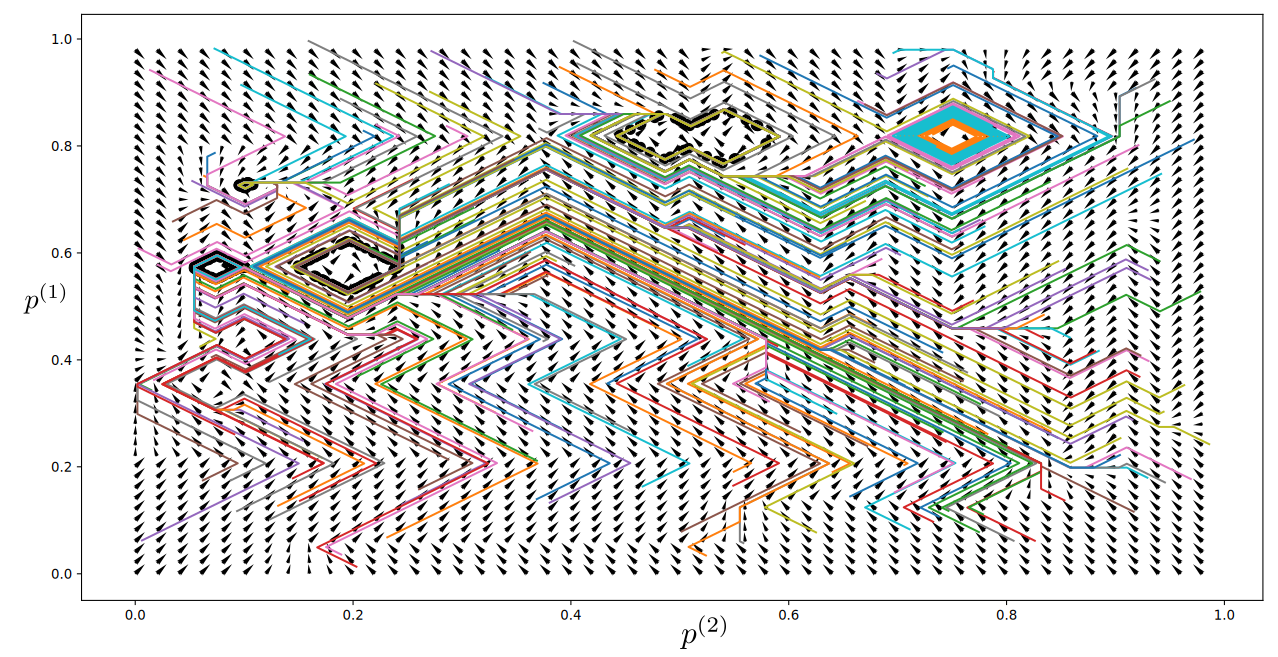
\includegraphics[width=\textwidth]{champ_006_t1.pdf}
\caption{Champ de déplacements de $\bmu\m{1},\bmu\m{2}$ lorsque les poids sont encore aléatoires, à $t=0$. En fonction de la position initiale des BMUs, la relaxation évolue vers un point fixe ou un cycle limite.}
\label{fig:champ_0}
\end{figure}


\begin{figure}
\centering
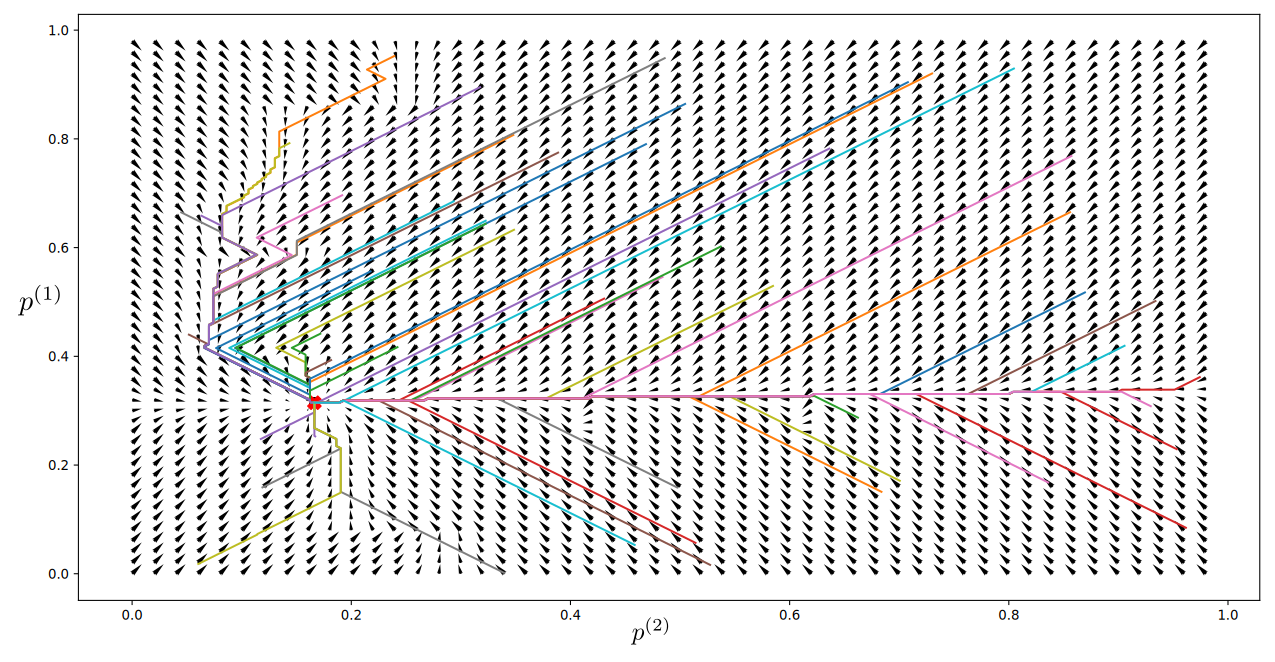
\includegraphics[width=\textwidth]{champ_006.pdf}
\caption{Champ de déplacements de $\bmu\m{1},\bmu\m{2}$ lorsque les poids sont organisés tels que représentés en figure \ref{fig:w006}, à $t=9999$. La relaxation évolue vers un point fixe pour l'entrée considérée.}
\label{fig:champ_9999}
\end{figure}

\subsection{Influence du pas de convergence}

Dans les expériences précédentes, on a utilisé un pas de convergence $\delta=0.05$. Une autre solution est de ne pas utiliser de pas de relaxation, c'est à dire, à chaque itération, déplacer le BMU $\bmu\m{i}$ directement à la position ou l'activité globale est maximale, au lieu de le déplacer de $\delta$ vers cette position.
L'évolution de la relaxation devient alors:
\begin{equation}
\forall i, \bmu\m{i}_{\tau+1} = p\star\m{i}_{\tau}
\end{equation}
En figure \ref{fig:diff_nopas}, on trace différentes trajectoires de relaxation, pour une même entrée. Ces relaxation sont effectués après l'apprentissage des données par l'architecture. Le processus de relaxation effectué pendant l'apprentissage n'utilise pas de déplacement $\delta$ non plus. 
On représente sur cette même figure les différences ${p\star}\m{1} - p\m{1}$ et ${p\star}\m{2} - p\m{2}$. La relaxation semble encore converger vers un point fixe.


\begin{figure}
\begin{minipage}{0.5\textwidth}
\includegraphics[width=\textwidth]{champ_X_009}
\end{minipage}
\begin{minipage}{0.5\textwidth}
\includegraphics[width=\textwidth]{champ_Y_009}
\end{minipage}
\caption{Trajectoires des relaxations $(\bmu\m{1}_{\tau},\bmu\m{2}_\tau)$ dans le champ des différences ${p\star}\m{1} - p\m{1}$ et ${p\star}\m{2} - p\m{2}$, lorsque la relaxation est effectuée sans utiliser de petits déplacements. Les tracés sont effectués après apprentissage. La relaxation semble encore converger vers un point fixe.}
\label{fig:diff_nopas}
\end{figure}

\subsection{Discussion}
Les parties \ref{sec:conv} et \ref{sec:cont} montrent que, lorsque les poids sont quelconques, la convergence de l'algorithme de relaxation n'est pas assurée; au contraire, la relaxation évolue dans $90 \%$ des cas vers une situation non convergente. Dans le cas étudié, il semble exister des zones de "point fixe", mais dues au hasard. La relaxation ne permet pas de trouver ces points. Pourtant, l'apprentissage des cartes, utilisant la relaxation comme recherche de BMU, permet une organisation des poids. Cette organisation, de plus, permet une meilleure convergence de la relaxation (convergence dans plus de $90 \%$ des cas).
On observe que la relaxation converge dans la plupart des cas à partir du moment où les poids externes sont organisés et présentent une continuité. Au début de l'apprentissage, même si la relaxation mène à des positions quelconques de BMUs, ces BMUs auront quand même des poids externes proches de la valeur de l'entrée. Le calcul de l'activité dépend en effet d'abord de l'activité externe de la carte : 
$$ a_g = \sqrt{a_e ( \beta a_e + (1-\beta a_c))}, \;\; \beta=0.5$$ 
L'organisation de la carte s'effectuera donc comme dans une carte classique. En effet, pour des poids aléatoires, de multiples positions de BMU sont possibles lors du calcul de la distance des poids à l'entrée. La disposition des poids et le choix du BMU n'influencent pas la propriété globale d'organisation d'une carte. Cette même observation peut s'effectuer ici.
Lorsque les poids externes présentent une continuité, la relaxation converge. 

